\documentclass[
    a4paper,
    12pt,
    oneside
]{report}

% Import packages
\usepackage{graphicx}
\usepackage{subfigure}
\usepackage{amsmath}  % Replaced latexsym with amsmath for symbols and mathematical operations
\usepackage[utf8]{inputenc}
\usepackage[english]{babel}
\usepackage{pdfpages}
\usepackage[
    backend=biber,
    style=ieee
]{biblatex} % IEEE style citations
\usepackage{csquotes}
\usepackage{url}
\usepackage[T1]{fontenc}
\usepackage{float}
\usepackage{palatino}
\usepackage{color}
\usepackage{algorithm}
\usepackage{algorithmic}

\setlength{\doublerulesep}{\arrayrulewidth}
% \setlength{\textwidth}{16cm}
% \setlength{\textheight}{24cm}
% \setlength{\hoffset}{-1.7cm} 
% \setlength{\voffset}{-1cm}
% \setlength{\topmargin}{-0.5cm} 
% \setlength{\footskip}{27pt}
\usepackage[a4paper, margin=2.5cm]{geometry}

\renewcommand{\baselinestretch}{1.3}
\linespread{1}

\usepackage{titlesec}
\titlespacing*{\chapter}{0pt}{-1\baselineskip}{1\baselineskip}
\titlespacing*{\section}{0pt}{\baselineskip}{0pt}

\usepackage{fancyhdr}
\usepackage{booktabs} 

\fancypagestyle{noheadrule}{
    \fancyhf{}
    \renewcommand{\headrulewidth}{0pt}
    \renewcommand{\footrulewidth}{0.5pt}
    \fancyfoot[L,LO]{\textit {FINAL PROJECT: Collective Transport using
    Decentralised Swarm Robotics}}
    \fancyfoot[R,RO]{\bfseries\thepage}
}

% Add bibliography file to document
\addbibresource{biblio.bib}

\begin{document}

% Cover
\begin{titlepage}
    \centering
    % \vspace*{1cm}

    {\LARGE \textbf{Final Project I}}\\[1cm]
    {\Huge \textbf{Collective Transport using Decentralised Swarm Robotics}}\\[1cm]

    
\includegraphics[width=0.4\textwidth]{assets/images/ise_logo.png}\\[1cm]
    
    \textbf{Submitted to the}\\[0.1cm]
    Project Committee appointed by the\\
    \textbf{International School of Engineering (ISE)}\\
    Faculty of Engineering, Chulalongkorn University\\[1cm]

    \textbf{Project Adviser}\\[0.1cm]
    Asst.Prof.Paulo Fernando Rocha Garcia, Ph.D.\\[1cm]

    \textbf{Submitted By}\\[0.5cm]
    \begin{tabular}{rl}
        6438067021 & Nattadon Tangsasom \\
        6438075021 & Ting-Yi Lin \\
        6438079621 & Tinapat Limsila \\
        6438118421 & Noppawan Srikhirin \\
        6438187721 & Mehul Sharma \\
    \end{tabular}\\[1cm]
    2/2024: 2147417 Final Project II\\
    Robotics and Artificial Intelligence Engineering (International Programme)\\
    International School of Engineering (ISE) Faculty of Engineering, Chulalongkorn University

\end{titlepage}


\thispagestyle{empty}
\pagenumbering{roman} \setcounter{page}{1}
\setcounter{secnumdepth}{11}
\setcounter{tocdepth}{3}
\renewcommand{\chaptermark}[1]{\markboth{Chapter ~\thechapter~:~#1}{}}
\fancyhf{}
\fancyhead[R,RO]{\bfseries\leftmark}
\fancyfoot[L,LO]{\textit {FINAL PROJECT: Collective Transport using
Decentralised Swarm Robotics}} 
\fancyfoot[R,RO]{\bfseries\thepage}
\fancypagestyle{plain}{
    \fancyhead{}
    \renewcommand{\headrulewidth}{0pt}
} 
\pagestyle{fancy}
\selectlanguage{english}
{\linespread{.8}\tableofcontents}
\newpage
\pagenumbering{arabic}
\titlespacing{\chapter}{0cm}{1cm}{2cm}

% Opening chapters
\chapter*{Abstract}

\paragraph*{}
This report serves as the proposal for our final project, titled "Collective Transport using Swarm Robotics." It covers various facets of our project, including the project concept, expected outcomes, project timeline, and potential benefits to the industry. Additionally, a comprehensive review of existing literature and a robust theoretical foundation are provided to substantiate our objectives.

\paragraph*{}
Structured into nine chapters, the report begins with an exploration of the research background and our objectives. The literature survey evaluates multiple research papers to identify relevant concepts, enhancing and applying them in innovative ways. Subsequent chapters delve into the development of the project concept, detailing the planning and execution strategy. A theoretical backup section fortifies our project methodology. The anticipated project outcomes are discussed, followed by the potential benefits to the industry. The report concludes by outlining each team member's contributions to the project.

\paragraph*{}
As a proposal for our final project, this report is intended to outline our plans and should not be considered as a finalized product. The comprehensive information provided across the nine chapters aims to furnish sufficient details for an effective project proposal.

\chapter{Introduction}

\paragraph*{}
This progress report aims to highlight the progress of our final project, \textbf{Collective Transport using Swarm Robotics}, with the evaluating criteria being the team individual contributions, as well as our pace in comparison to the ideal schedule. The ideal schedule can be represented by the project Gantt Chart (Figure \ref{fig:gantt_chart}).

\paragraph*{}
According to Figure \ref{fig:gantt_chart}, we are exploring three major sub-tasks during this iteration of the project schedule. These three tasks are: \textbf{Communication in the Swarm} (Task 1.1), \textbf{Object detection using Computer Vision} (Task 1.2), and \textbf{Simple Simultaneous Localization and Mapping} (Task 1.3). These tasks are planned to span for the entire month of September. Two team members, one team member, and two team members are assigned to each task, respectively.

\begin{figure}[H]
    \centering
    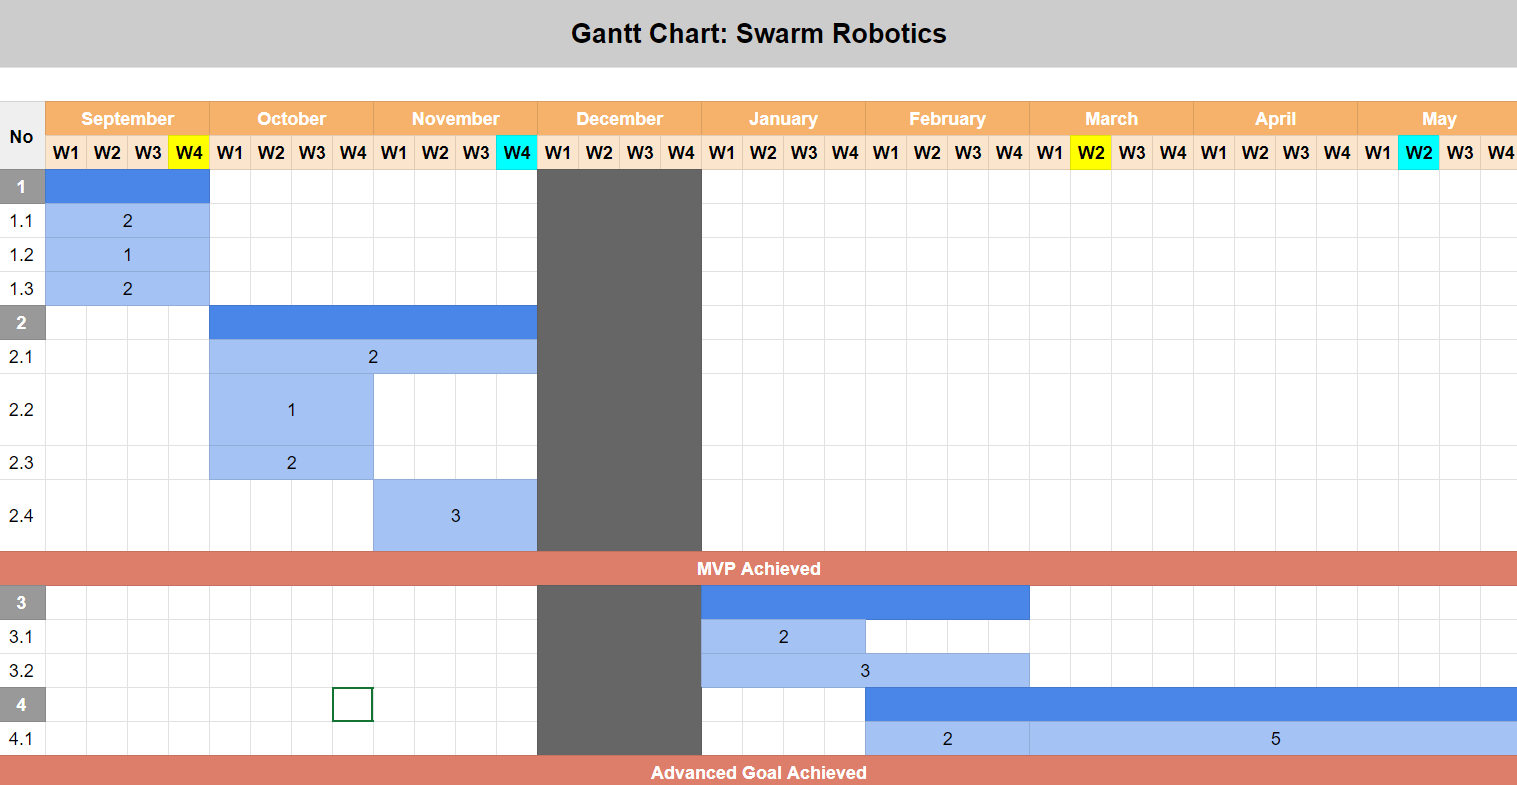
\includegraphics[width=1\linewidth]{progress_report_1/assets/images/introduction/gantt_chart.png}
    \caption{Project Gantt Chart}
    \label{fig:gantt_chart}
\end{figure}

\chapter{Literature Survey and Review}

\section{Coordination}

\paragraph*{}
Swarm robotics solution is a design architecture that obtains inspirations from biological interactions; thus, they should operate autonomously to solve problems rather than relying on a central authority\cite{turkler2022usage}. This decentralised approach is also crucial to achieve increased resilience and flexibility given a complex environment of deployment\cite{das2024bio}.

\paragraph*{}
Communication protocols can be categorised into two principal types depending on the nature of information transmission: Direct communication and Indirect communication\cite{das2024bio}. Direct communication refers to robotic agents that are able to coordinate via networked communication. Direct communication use cases are highlighted in many studies.

\paragraph*{}
Ibrahim et al. \cite{ibrahim2024enhancing} studied direct communication to determine the optimal distance for robotic agents to achieve consensus. Three strategies were tested within a 50 cm range: Close-neighbour, Far-neighbour, and Rand-neighbour. Close-neighbour excels in stable environments but performs poorly in complex ones. Both Close-neighbour and Far-neighbour introduce bias, reducing accuracy. Rand-neighbour, which randomly selects swarm members for communication, proved superior due to efficient information flow and minimal bias. This strategy can be one of our key designs for swarm communication in this project.

\paragraph*{}
Ayari and Bouamama\cite{ayari2023evolutionary} and Perera et al.\cite{perera2022integrating}, S et al.\cite{sr2023control} and Z. Wang et al.\cite{wang2024decentralized} conducted studies to promote robots’ actions based on their sensory observations and objectives. S et al.\cite{sr2023control} proposed a Multi-Agent Deep Deterministic Policy Gradient (MA-DDPG), an observation-based decision making flow with an architectural twist, where there is a central swarm manager that evaluates decentralized agents' reinforcement learning for optimal rewards. Z. Wang et al.\cite{wang2024decentralized} proposed increasing sensory inputs from both visual data and communication for redundancy, which highly aligns with the proposed swarm system.

\paragraph*{}
Yasser et al.\cite{yasser2024optimized} expanded more on Clustered Dynamic Task Allocation (CDTA), an approach to dynamically assign tasks based on swarm state and the environment \cite{nedjah2021communication}, for the purpose of increasing the velocity of swarm communication. They proposed CDTA-CL (Centralized Loop) and CDTA-DL (Dual Loop). CDTA-CL sends information to the leader for computation, while CDTA-DL compares information before sending it to the leader. CDTA-DL outperformed CDTA-CL, increasing speed by 75.976\% compared to 54.4\%. CDTA-DL will be considered as a design pillar for this project.

\paragraph*{}
In addition to direct communication improvements, indirect communication, known as Stigmergy, also plays a significant role in swarm intelligence. This concept involves individual robot actions modifying the environment, impacting the decision-making of other robots. For example, construction robots can leave blocks and materials to signal ongoing work\cite{das2024bio}. This is an intriguing notion to consider in the interaction of the swarm system.

\paragraph*{}
For effective communication, especially in interdependent tasks, robots need to be aware of each other and task requirements. Semantic communication, where contextually relevant data is prioritized, is necessary\cite{beck2023swarm}. The balance between communication and context must align with task demands. High sensory data tasks require reliable, real-time communication, while tasks with lower communication demands can prioritize contextually relevant information\cite{zhang2021cooperative}.

\section{Object Detection}

\paragraph*{} 
Object detection is an essential component of this project, enabling each member of the swarm to perceive their environment and effectively interact with various targets. Traditional 2D object detection methods face challenges in dynamic and complex settings, where accurate estimation of size, distance, and position is critical \cite{hybridframework2023}. To address these issues, integrating a camera sensor with a LiDAR system offers a reliable solution for 3D object detection \cite{janai2020}, enabling precise measurement of the distance to the target as well as its dimensions.

\paragraph*{} 
Object detection algorithms are typically classified into three categories based on the sensors utilised: camera-based algorithms, LiDAR-based algorithms, and LiDAR-camera fusion algorithms. The first category involves the use of a monocular camera for detection. Object detection with monocular cameras can be achieved through either traditional methods or deep learning-based approaches.

\paragraph*{} 
Traditional methods, such as the Scale-Invariant Feature Transform (SIFT), identify key points in images that are invariant to rotation and scaling, making them suitable for recognising objects under various transformations \cite{lowe2004distinctive}. Another widely used traditional approach is the Histogram of Oriented Gradients (HOG), which captures the distribution of gradient orientations within an image \cite{dalal2005histograms}. Both SIFT and HOG have been instrumental in earlier object detection tasks due to their effectiveness in identifying salient features.

\paragraph*{} 
In contrast, deep learning-based approaches have revolutionised object detection by surpassing traditional methods in terms of accuracy and adaptability. Prominent algorithms such as YOLO (You Only Look Once), SSD (Single Shot MultiBox Detector), and Faster R-CNN offer unique advantages and trade-offs \cite{sachan2019object}. YOLO is renowned for its real-time processing capabilities, making it well-suited for applications requiring high-speed detection without significant compromises in accuracy \cite{redmon2016you}. Faster R-CNN employs a two-stage process that prioritises detection accuracy, although at the cost of slower inference speeds, making it ideal for tasks where precision is critical \cite{ren2015faster}. Meanwhile, SSD strikes a balance between speed and accuracy by using a single-shot detection mechanism with moderate computational requirements \cite{liu2016ssd}.

\paragraph*{} 
A comparison of these three models is shown in Table \ref{tab:performance_metrics}, focusing on their speed, precision, and adaptability. The evaluation results demonstrate that YOLOv8 excels in multi-object detection, combining high accuracy with balanced speed and efficiency. This makes it a preferred choice for real-time applications due to its lower hardware demands \cite{kaliappan2023real}.

\begin{table}[!h]
    \centering
    \begin{tabular}{| p{3.5cm} | p{3cm} | p{4cm} | p{3.5cm} |}
        \hline
        Algorithms  & Recall Value  & Mean Average Precision (mAP@0.5)  & Precision \\ \hline
        YOLOv8  & 1.00  & 98.7\%  & 96.77\% \\ \hline
        SSD  & 0.65  & 77\%  & 89\% \\ \hline
        Faster R-CNN  & 0.67  & 59\%  & 77\% \\ \hline
    \end{tabular}
    \caption{A comparative analysis of YOLOv8, SSD, and Faster R-CNN based on key performance metrics, including Recall Value, Mean Average Precision (mAP@0.5), and Precision \cite{kaliappan2023performance}.}
    \label{tab:performance_metrics}
\end{table}

\paragraph*{} 
Monocular camera-based object detection relies solely on 2D image data to identify objects and approximate their depth and location using visual cues. While such cameras are effective in detecting colour and texture, estimating depth accurately often requires stereo vision or additional sensors.

\paragraph*{} 
LiDAR-based object detection algorithms provide precise spatial and depth information in the form of 3D point clouds, making them highly effective for localising objects in complex environments, particularly under poor lighting conditions where cameras may struggle \cite{geiger2013vision}. LiDAR-based approaches can be broadly categorised into point-based and voxel-based methods.

\paragraph*{} 
Point-based methods operate directly on raw 3D point clouds, leveraging their inherent spatial accuracy without converting the data into grids or images. For example, PointNet employs a shared Multi-Layer Perceptron (MLP) to extract features from individual points and aggregates these using max-pooling to capture global context \cite{qi2017pointnet}. PointNet++ enhances this approach by introducing hierarchical feature extraction to capture local geometric features, enabling better performance in cluttered or large-scale environments \cite{qi2017pointnet++}.

\paragraph*{} 
Conversely, voxel-based methods transform raw point clouds into structured voxel grids, allowing for efficient feature extraction using 3D convolutional neural networks (CNNs). A notable example is VoxelNet, which divides the 3D space into voxels and extracts features using PointNet-inspired architectures, followed by 3D CNNs for detection \cite{zhou2018voxelnet}. Advances such as SECOND improve computational efficiency by optimising voxel representations and employing sparse convolutions \cite{yan2018second}.

\paragraph*{} 
While LiDAR provides unparalleled depth and spatial accuracy, it lacks the rich texture and colour information necessary for tasks such as object classification and semantic segmentation. LiDAR-camera fusion addresses these limitations by combining the strengths of both sensors. Models such as Frustum PointNet project 2D image proposals onto LiDAR point clouds, improving object localisation and classification \cite{qi2018frustumpointnet}. Frameworks like MV3D and AVOD demonstrate how fusing RGB images and LiDAR data achieves significant performance improvements \cite{ku2018mv3d}.

\paragraph*{} 
The integration strategy for LiDAR-camera fusion is crucial and can be classified into three categories:

\begin{itemize}
    \item \textbf{Early Fusion}: Aligns raw LiDAR point clouds with camera frames for unified processing \cite{ku2018mv3d}.
    \item \textbf{Mid-Level Fusion}: Merges features extracted separately from LiDAR and camera data \cite{chen2017avod}.
    \item \textbf{Late Fusion}: Combines decisions made by independent LiDAR and camera models \cite{qi2018frustumpointnet}.
\end{itemize}

\paragraph*{} 
Another critical task in object detection is determining the position and orientation of objects in the environment. Accurate pose estimation enables robots to interact effectively with their surroundings for tasks such as navigation, manipulation, and object placement \cite{paul2021object}. Pose estimation methods are broadly categorised into model-based approaches, such as Iterative Closest Point (ICP) \cite{yuan2023accurate}, and learning-based methods, including PoseNet \cite{kendall2015posenet} and PVNet \cite{peng2019pvnet}.

\paragraph*{} 
Common benchmarks for evaluating pose estimation algorithms include datasets such as LINEMOD and YCB-Video, which offer annotated images and depth maps under varying poses and lighting conditions. However, challenges such as dynamic environments, real-time constraints, and robust performance under occlusions remain areas for further research \cite{chen2022occlusion}.

\section{SLAM}

\paragraph*{}
SLAM, or Simultaneous Localization and Mapping, is a widely spread algorithm for navigation in the field of mobile robotics because of the exponential improvement in computer processing speed and the accessibility of sensors such as cameras and LiDAR \cite{barbadekar2023exploring}. Using SLAM, a mobile robot can construct an internal environment map while simultaneously using the map to estimate its location without needing predefined knowledge of area \cite{durrant2006simultaneous}.

\paragraph*{}
Environment mapping is one of the vital techniques in SLAM. The algorithm consists of building a mathematical model for the spatial information of an actual environment, which encapsulates the necessary information for navigation and interaction. However, as for the SLAM technique, additional requirements are needed; the mathematical model must be able to represent the robot’s state and the position of landmarks relative to the robot’s location \cite{durrant2006simultaneous}. Hence, the challenge with the requirements is that the robot must perform the localization and the mapping simultaneously.

\paragraph*{}
Given these complexities, the backbone of all principal SLAM methods is the utilization of these SLAM frameworks consisting of odometry, landmark prediction, landmark prediction, landmark extraction, data association, and matching, pose estimation, and map update \cite{chong2015sensor}.

\paragraph*{}
Building on this, situational awareness becomes an extreme component of SLAM, the precision and accuracy of the robot's perception play a huge role in defining the characteristics of other variations of the SLAM implementation. Therefore, a thorough understanding of advantages and disadvantages of each common perception device is an imperative concept not just for the robot’s components but also the structure of the SLAM’s backend algorithm. 

\paragraph*{}
Firstly, acoustic sensors are widely used across the preliminary stage of SLAM implementations to minimize the pose drift with time, with most of the sensors being SONAR, or Sound Navigation and Ranging \cite{udugama2023evolution}. These sensors are well operated in dark environments, as well as dusty and humid, due to their insensitivity towards illumination and opaqueness \cite{sahoo2019advancements}. 

\paragraph*{}
Secondly, LiDAR, or Light Detection and Ranging Sensor, is relatively similar to an ultrasonic sensor in terms of functionality \cite{udugama2023evolution}. However, LiDAR uses electromagnetic waves as a radiation reference instead of acoustic waves. A LiDAR renders a 3-dimensional representation of its surroundings known as the Point Cloud \cite{bisheng2017progress}. The strength of LiDAR is that the sensor can provide 360 degrees of perception with high precision \cite{cadena2016past}.

\paragraph*{}
Thirdly, depth cameras' mechanism works based on the illumination of the site with infrared light and measures the time-of-flight \cite{langmann2012depth}. Comparing the range of measurement and accuracy, a depth camera performs poorer than a 3D LiDAR scanner because the depth camera can only acquire data within a limited range of field of view; moreover, environmental factors may affect the accuracy of the depth camera; for example, the depth camera’s output is susceptible to certain materials of surfaces, such as reflective or transparent materials \cite{peng2023depth}. However, a depth camera is still a popular option for SLAM as it's a relatively economical device compared to its relatives, 3-D LiDAR, for instance.

\paragraph*{}
Ultimately, event-based cameras present the local bitmap-level motion alterations to an event that took place, which is different from conventional framing-based cameras \cite{udugama2023evolution}. The new technique has gained popularity more recently in the field of SLAM as an event-based camera yields more efficient computational performance and better overall accuracy \cite{huang2023event}.

\paragraph*{}
After reviewing the different sensors and addressing technological advancements available in today’s world, it is crucial to understand how researchers have implemented those ideas to different variations of SLAM. This understanding helps in overcoming challenges and limitations that their predecessors had faced and set new standards for new research frontiers. Moreover, it becomes essential to effectively classify those SLAM variations under different criteria.

\paragraph*{}
Li et al.\cite{li2024object} perfectly encapsulated how SLAM techniques can be classified: 

\paragraph*{}
Simultaneous Localization and Mapping (SLAM) techniques can be categorized by using different factors. Firstly, they can be divided into categories based on the type of sensors employed. They may include vision-based SLAM using cameras, LIDAR-based SLAM using LIDAR sensors, and RGB-D SLAM, which combines RGB cameras with depth sensors. Secondly, feature-based SLAM, which tracks distinguishing characteristics and direct SLAM, which executes mapping intensity or depth directly can be considered as different categories. Thirdly, the estimated approach, such as filter-based SLAM, which uses filters such as Particle Filter and graph-based SLAM, which is formulated as a graph optimization problem, provides another classification criterion. Finally, SLAM can be categorized based on time synchronization, with offline SLAM processing data in batches after collection and online SLAM estimating pose and map incrementally in real-time.

\paragraph*{} 
LiDAR-based SLAM is one of the most widely used variations of SLAM, leveraging LiDAR sensors to accurately localize itself while simultaneously building a map of its surroundings. This approach uses registration algorithms, such as Iterative Closest Point (ICP), to estimate relative transformations between point clouds during operation \cite{gu2020review}. Feature-based algorithms, such as LiDAR Odometry and Mapping (LOAM), further enhance this process by representing 2D or 3D point cloud maps as grid maps \cite{zhang2014loam}. LiDAR’s ability to function reliably in diverse lighting conditions and environments makes it particularly suitable for SLAM applications in challenging scenarios.

\paragraph*{} 
An evolution of SLAM techniques is the use of graph-based SLAM, which focuses on optimizing a graph representation of the robot's trajectory and surrounding environment. In graph SLAM, nodes represent robot poses or landmarks, while edges denote constraints, such as relative transformations obtained from sensors like LiDAR or odometry \cite{grisetti2010tutorial}. The optimization of this graph structure, often performed using techniques like the Gauss-Newton method, allows for accurate loop closure and global consistency \cite{kummerle2011g2o}.

\paragraph*{} 
Another emerging trend in SLAM is the integration of multi-sensor data to overcome the limitations of individual sensing modalities. For example, algorithms such as FAST-LIO combine LiDAR data with inertial measurements from IMUs to improve robustness and accuracy \cite{xu2021fast}. Multi-sensor approaches ensure better adaptability to real-world conditions, enabling more precise localization and mapping.

\paragraph*{} 
Cartographer is a versatile open-source SLAM library developed by Google, designed to handle 2D and 3D SLAM applications. It is particularly known for its robust pose graph optimization and real-time performance, leveraging submapping techniques to efficiently manage computational resources. Cartographer uses LiDAR, IMU, and odometry data to create globally consistent maps by detecting and correcting loop closures, making it suitable for indoor and outdoor mapping tasks \cite{hess2016real}. Its modular architecture allows seamless integration into various robotic platforms, making it a popular choice for research and industry applications.

\paragraph*{} 
Another noteworthy SLAM framework is the SLAM Toolbox, an advanced open-source library tailored for ROS 2. It provides tools for lifelong mapping, localization, and pose-graph optimization. SLAM Toolbox supports features like merging maps, multi-session mapping, and robust handling of large-scale environments. Its loop closure detection and optimization capabilities enhance global consistency, ensuring accurate localization in dynamic and complex settings \cite{macenski2021slamtoolbox}. This makes SLAM Toolbox ideal for applications that require long-term operation in evolving environments, such as warehouses and public spaces.

\section{Collective Movement}

\paragraph*{}
In the domain of swarm robotics, collective movement coordination and dynamic role assignment are crucial for enabling robots to work together efficiently. Research on coordinated motion in swarms often emphasises the need for algorithms that allow robots to adapt their roles and behaviours in real-time. For example, the study on "Efficient Strategies for Coordinated Motion and Tracking in Swarm Robotics" is a comprehensive overview of various coordination algorithms, contrasting different techniques for multi-robot collaboration. 

\paragraph*{}
The first coordination algorithm mentioned is the leader-follower model. This algorithm is rather straightforward in the sense that one or more robots are designated to guide the swarm while the other robots adjust their positions. The leader can be pre-programmed or autonomously chosen depending on the path while the followers maintain a set distance and set angle. This model as mentioned before is simple to apply while also being centralised providing clear direction for the followers. Additionally, the followers do not need the full knowledge of the environment meaning that this model can be scalable. However, this swarm being centralised means that it is prone to a single point of failure and having reduced flexibility \cite{mehta2024robust}. This model would only work well for a simple structured environment with predefined paths which unfortunately does not match with our objectives.

\paragraph*{}
Another coordination algorithm is the potential fields algorithm. This algorithm is based on virtual forces with each robot in the swarm being treated as a particle that is influenced by virtual forces exerted by other robots, obstacles and targets. These forces can attract or repel each other. The object is for the robot to be “pulled” towards the goal while avoiding collisions. This model has a couple advantages; namely: Decentralised control as each robot moves autonomously based on the forces acting on it, and smooth movements. However a couple of challenges come with it as well. One challenge is the possibility of the robot being stuck in a local minimum where virtual forces cancel each other out. Secondly, proper fine tuning of the force parameters is required to prevent the robot from oscillating \cite{martinez2023swarm}. Overall this approach could be useful for environments with many obstacles where smooth and continuous navigation can be important.  The third algorithm offered is the virtual force algorithm which is similar to the potential fields algorithm but with more constraints thereby being ineffectual to our project \cite{udugama2023evolution}. 

\paragraph*{}
When comparing these three algorithms above, potential field algorithm and virtual force algorithm are decentralised while the leader-follower model is centralised. While the leader-follower model offers a simple, scalable nature, it introduces a single point of failure. In contrast, the potential fields algorithm offers a more decentralised approach, which is better suited for dynamic environments but requires careful turning to avoid local minima.

\paragraph*{}
In swarm robotics, dynamic role assignment plays a crucial role in enabling robots to adapt their behaviours and tasks in real-time. One common method is insect-inspired behaviour, which mimics the role distribution seen in social insect colonies \cite{bonabeau1997adaptive}. In this approach, robots assume roles based on simple, local rules, such as task demand or proximity to a target, without centralised control. This method offers high scalability and robustness, as robots can seamlessly take on different tasks as needed, making it suitable for large swarms. However, its reliance on local information can sometimes lead to suboptimal task assignments, particularly in complex environments where global awareness might be needed.

\paragraph*{}
On the other hand, market-based approaches \cite{brambilla2012property} use a more structured mechanism where robots bid for tasks based on their capabilities and availability. This ensures that tasks are allocated to the most suitable robots, leading to more efficient task execution. However, the bidding process requires communication between robots, which may introduce delays and increase system complexity. While market-based approaches tend to be more optimal for task allocation, they may not scale as easily as insect-inspired methods, especially in large or dynamic environments where constant communication is challenging.

\paragraph*{}
Decentralised control in swarm robotics offers several key advantages, particularly in terms of scalability, robustness, and adaptability \cite{st-onge2023swarm}. In decentralised systems, each robot operates autonomously, relying on local information and interactions with neighbouring robots, which eliminates the need for a central controller. This allows the swarm to scale more easily, as adding more robots does not increase the computational or communication burden on a single entity. Additionally, decentralised systems are more robust, as the failure of one or more robots does not compromise the entire system; each robot can continue functioning independently. This is particularly advantageous in dynamic or unpredictable environments, where flexibility and fault tolerance are critical.

\paragraph*{}
In contrast, centralised control systems rely on a single controller to manage all robots, which creates a bottleneck as the number of robots increases. Centralised systems can suffer from single points of failure—if the controller fails, the entire system may halt. Moreover, communication delays and computational limits can hinder real-time performance in larger systems. While centralised control offers more efficient coordination in smaller, simpler environments, decentralised control is better suited for real-world applications where scalability and resilience are essential for handling complex and dynamic tasks.

\paragraph*{}
Despite significant advancements in swarm robotics and coordination algorithms, there remain notable gaps in applying these methods to practical, real-world environments such as cleaning tasks. Most research on algorithms like potential fields, leader-follower models, and market-based role assignment has focused on simulations or controlled environments, which often lack the complexity and unpredictability found in real-world scenarios. For instance, limited work has been done on integrating these algorithms with sensor-rich, dynamic settings where robots must navigate cluttered spaces, identify and manipulate diverse objects, and coordinate in real-time without centralised control. Additionally, the scalability of these systems is often not tested in practical, large-scale environments, such as a commercial building cleaning system, where communication constraints, battery life, and real-time decision-making are crucial factors.

\paragraph*{}
Our project aims to address these gaps by developing a swarm of cleaning robots that leverages C-SLAM for real-time mapping and localization, along with a hybrid role assignment approach that adapts based on task proximity and robot capabilities. By testing in realistic environments with obstacles, diverse object types, and multiple robots working simultaneously, our project will not only explore the robustness of these algorithms but also refine them for practical deployment in domestic and commercial cleaning. This will bridge the gap between theoretical research and real-world application, offering a scalable and adaptive solution for multi-robot systems.


% Content chapters
\chapter{Communication}

\paragraph*{}
This chapter details the exploratory results for the sub-task \textbf{Communication in the Swarm}. This task has been tackled under the assumption that the \textit{swarm fleet are capable of object detection}, which is a necessary premise to parallelize the workload as another group member is working on it. Some other vital constraints include:

\begin{itemize}
    \item \textbf{Robots are stationary} \\
    This is assumed because we can temporarily exclude motor control for simplicity
    \item \textbf{Robots are on fixed coordinates configured by the user} \\
    This is assumed because robots can communicate their coordinates to other fleet members and the assumption offers an easy method to check for the correctness in their communication.
    \item \textbf{Start with 5 robots during simulation} \\
    This constraint is to minimize the complexity in the environment
\end{itemize}

\paragraph*{}
After thorough consideration and evaluation, the best simulating environment for this specific communication task is Webots from Cyberbotics. Webots provide the PROTO mechanism for developers to build and reuse complex objects. This allows us to simulate and test our assumptions upon pre-built objects, such as 
TurtleBot. 

\begin{figure}[H]
    \centering
    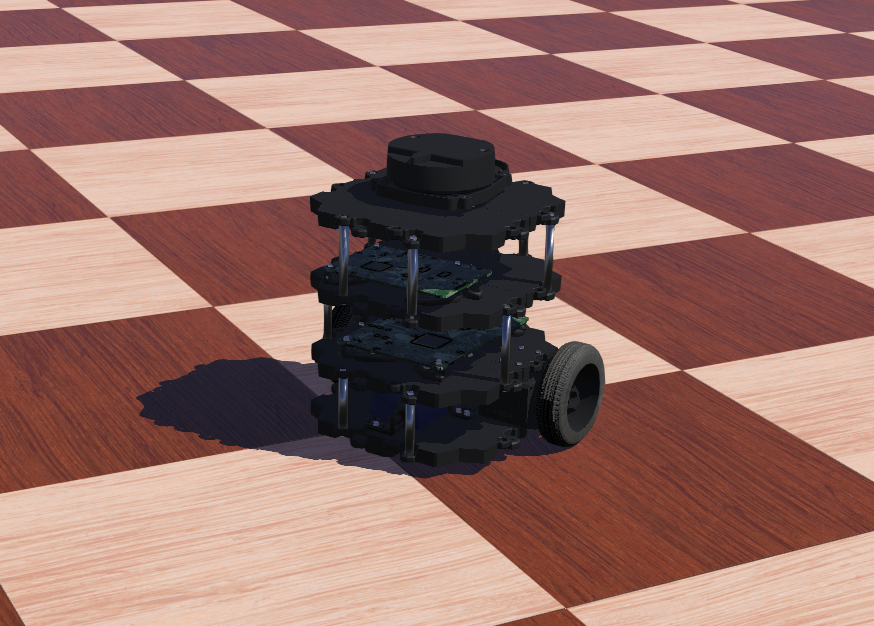
\includegraphics[width=0.4\linewidth]{assets/images/communication/environment/turtlebot.png}
    \caption{TurtleBot 3 Burger in Webots}
    \label{fig:turtlebot}
\end{figure}

In webots, the version of the TurtleBot given in the PROTO nodes is the Burger model of the third version of the TurtleBot robot Figure \ref{fig:turtlebot}.  Moreover, the TurtleBot has two functioning motors and a 360-degree distance sensor, allowing it to do simple navigation. However, using TurtleBot alone is inadequate to simulate the communication framework. Therefore, three more basic nodes are added to the TurtleBot object, which are the following: Firstly, the GPS node (Figure \ref{fig:GPS}), this module is installed to obtain the robot's position in the simulated world. This direct approach is used because the localization and mapping process is not accounted for in this testing. Secondly, the Emitter node (Figure \ref{fig:Emitter}), this module is added to the robot to model a broadcast behavior. Additionally, Webots allows the developer to configure the properties of the Emitter Class; for instance, the emission range. Thirdly, the Receiver node (Figure \ref{fig:Receiver}), this module is connected as an accompaniment to the Emitter Class, because the Emitter node does not support both emitting and receiving functionalities. The receiver listens for incoming data packets and appends them to the tail of a queue. Moreover, incoming data packets will be discarded if the receiver's buffer size is exceeded. With all the

\begin{figure}[!htb]
    \minipage{0.32\textwidth}
        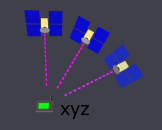
\includegraphics[width=\linewidth]{assets/images/communication/devices/gps.png}
        \caption{GPS node}\label{fig:GPS}
    \endminipage\hfill
    \minipage{0.32\textwidth}
        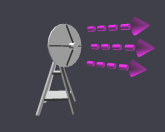
\includegraphics[width=\linewidth]{assets/images/communication/devices/emitter.png}
        \caption{Emitter node}\label{fig:Emitter}
    \endminipage\hfill
    \minipage{0.32\textwidth}%
        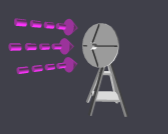
\includegraphics[width=\linewidth]{assets/images/communication/devices/receiver.png}
        \caption{Receiver node}\label{fig:Receiver}
    \endminipage
\end{figure}

\paragraph*{}
The main approach to communication in the swarm would be to gain awareness over robotic members in the swarm system and finding consensus within the swarm before any further follow-up actions are taken. In case of an object getting detected, the first robot that detects the object would act as the task master, supplying other robots in the swarm with the object's coordinates. Consensus is essential for this use case because every swarm members have to agree on the object detection before any actions. Therefore, we are utilizing modes to build a central template code to operate the swarm. There are two main modes for the swarm: \textbf{Idle} mode and \textbf{Consensus} mode.

\paragraph*{}
The \textbf{Idle} mode entails the period where fleet members are setting themselves up by communicating their \textbf{identifiers} and their \textbf{coordinates}, which the receivers store as internal dictionaries. Figure \ref{fig:idle_mode} displays the functional instance where the turtlebots in the environment are aware of other members and their respective coordinates and test-print them on console.

\begin{figure}[H]
    \centering
    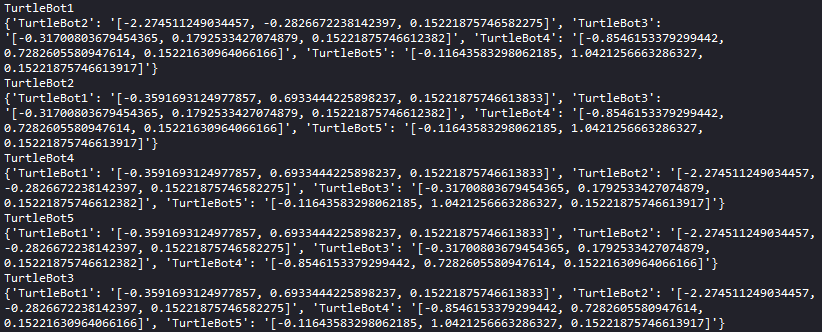
\includegraphics[width=1\linewidth]{assets/images/communication/outputs/idle_mode.png}
    \caption{Idle Mode}
    \label{fig:idle_mode}
\end{figure}

\paragraph*{}
The \textbf{Consensus} mode occurs when an object is "detected" by any of the swarm members. After the detection, the robot which identifies the object will switch its mode to Consensus and save the object's coordinates. Consequently, it will communicate to other members of the present object, readying them for any subsequent actions. In this test case, a set of object coordinates is manually supplied to one of the members after four seconds. Figure \ref{fig:consensus_mode} shows \textit{TurtleBot2}, a member in the environment, receiving the set of coordinates and communicating to the swarm that it is the task master and the location of the object, thereby bumping other robots' modes to Consensus mode.

\begin{figure}[H]
    \centering
    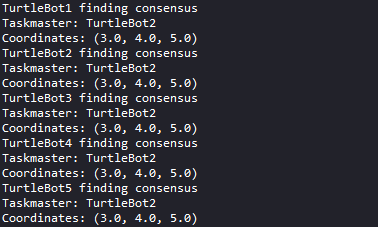
\includegraphics[width=0.6\linewidth]{assets/images/communication/outputs/consensus_mode.png}
    \caption{Consensus Mode}
    \label{fig:consensus_mode}
\end{figure}

\paragraph*{}
This approach can be improved by planning for worst-case-scenarios in advance. To expand further, this can be from preventing any race conditions occurring from the consensus mode, and including an extra verification step after communication. However, a potential challenge with the verification step is that robotic communication is extensive; having additional communication demands should be in balance with the available resources the robots allow.

\paragraph*{}
Additionally, the \textbf{application layer} is currently sending and receiving:

\begin{itemize}
    \item Robot's identifier
    \item Robot's coordinates
    \item Object coordinates
\end{itemize}

We will potentially require more information to be transmitted with additional requirements from other modules, which is another area for further improvements.

\chapter{Simple Robot Formation}

\paragraph*{}
This chapter records the exploratory endeavors into the realm of swarm robotics path planning in an attempt to build a formation around an "object". A brief recapitulation of the reason we require an object is because our end goal is to perform collective transportation using swarm robotics.

\paragraph*{}
In the process of building a swarm formation, computations for the desired coordinates where the swarm units should be moving to (later referenced as \textbf{"target coordinates"}), and the desired path the members can take in order to move towards the goal are essential. The key parameters for this calculation include: the \textbf{radius} where the swarm should place itself around the object, swarm fleet \textbf{member count}, \textbf{current coordinates} for the swarm, and target \textbf{object coordinates}.

\paragraph*{}
The member count is a vital initial point since it will be used to compute the angle \(\theta\) between each set of target coordinates using the following formula:

\[\theta = (2\pi / n) * i\]

\begin{description}
    \item[where:]
    \item \(\theta\) = angle between each set of target coordinates (in radians)
    \item \(n\) = swarm system member count
    \item \(i\) = member identifier (e.g. 0 to 4 for a swarm fleet of 5 members)
\end{description}

\paragraph*{}
Currently, the formation is determined by utilizing a given radius for the swarm robotic members to attempt to surround. In accordance with the member count providing the angle, the individual target coordinates for each robot can be calculated using an adaptation from the Pythagorean Theorem. 

\[x' = x + rcos\theta\]
\[y' = y + rsin\theta\]

\begin{description}
    \item 
    \item[where:]
    \item \((x, y)\) = robot's present coordinates
    \item \((x', y')\) = target \((x, y)\) coordinates
    \item \(r\) = radius
\end{description}

\paragraph*{}
The target coordinates at this stage would often result in floats; therefore, it is necessary to round the numbers and record the margins of error to snap the coordinates to a grid system. With the resulting calculation of the target coordinates, it is sufficient to proceed to the next stage, which is \textbf{path planning}. The path planning algorithm follows a simple \textbf{"Avoid paths that cause conflicts, but if all paths cause conflicts, pause before continuing"} rule. Hence, recording the paths and the timestep the movement will happen is crucial. The code for the algorithm is provided in Figure << replace with algorithm.

\paragraph*{}
With the attached algorithm, the console output for the functional instance of the algorithm is also provided (Figure \ref{fig:formation_console_output}). As can be seen, during the intended movement for robot2 and robot3, there is a conflicting movement in \textit{timestep 2} at the \textit{coordinates (3, 3)}. Therefore, robot3 halts for a single timestep before continuing. This is designed so that robots will not take unnecessary detours and create environment variabilities.

\begin{figure}[H]
    \centering
    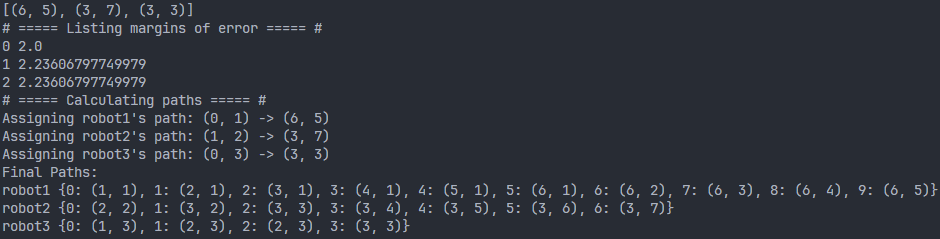
\includegraphics[width=1\linewidth]{assets/images/formation/console_output.png}
    \caption{Console Output}
    \label{fig:formation_console_output}
\end{figure}

\paragraph*{}
Nevertheless, this path planning algorithm still contains a glaring flaw. It currently does not consider obstacles in the environment. This can be seen as a room for improvement; or perhaps other modules can assist in offsetting this current drawback.

\chapter{Object Detection}

\paragraph*{}
The object detection system initially developed in the previous semester successfully detected a yellow cylinder, generated a bounding box around it, aligned the box’s center with the camera frame, and measured the distance between the robot and the object using the camera’s focal length. However, this implementation relied on the assumption that the cylinder’s dimensions were known, and LiDAR had not yet been integrated. Additionally, the scope of object detection was refined from hexagonal prisms and cubes to cylinders to eliminate the need for pose estimation and edge detection, which would otherwise introduce additional computational complexity for dynamic object grasping.

\paragraph*{}
In transitioning to real-world implementation, several modifications were made to the object detection workflow. The system now identifies three distinct objects: a yellow, a blue, and a red cylinder, each differing in size. At this stage, only a single object is placed in the arena at a time, with detection based primarily on colour. Once detected, the system generates a bounding box around the object, and its distance and size are measured using an S3 RPLiDAR. To enhance accuracy, multi-sensor fusion between the camera and LiDAR is employed. By leveraging the camera’s horizontal field of view (FOV), the system maps the bounding box’s pixel range to the corresponding angle and retrieves the appropriate LiDAR data based on the robot’s odometry.

\paragraph*{}
The current implementation has successfully demonstrated the ability to detect objects based on color while filtering out reflections from the floor. Initial testing was conducted under controlled lighting conditions, including illumination from the left, right, front, and back. The presence of vibrations caused by the camera mount during movement did not significantly affect detection performance. However, at this stage, accuracy assessments are still based on visual inspection, and further validation will be conducted once the model undergoes proper calibration with the sensors. Overall, progress remains on schedule and aligns with the expected timeline, with each milestone being achieved as planned.

\paragraph*{}
In measuring distance and size, image distortion remains a key factor influencing accuracy, as the system must correctly map the detected object’s bounding box angle to real-world coordinates. Since the object’s height does not contribute to measurement calculations, vertical calibration data from the camera has been omitted. Additionally, the top 30 degrees of the camera frame is cropped to remove potential noise and prevent false detections of unintended objects or individuals outside the arena.

\paragraph*{}
One of the primary challenges encountered in this phase is object occlusion, where multiple objects appearing in the frame can lead to overlapping bounding boxes. In such cases, the robot is required to reposition itself to separate the detected objects and ensure accurate size measurements without interference. Another challenge is ensuring reliable color detection under varying lighting conditions, as different light sources and angles can affect how the camera perceives object colors. Additionally, image distortion presents difficulties in mapping the bounding box to the correct position in relation to the LiDAR data. These obstacles are being addressed through careful calibration, adjustments in object positioning, and improvements to the detection algorithm to enhance its robustness against occlusion and lighting variations.

\paragraph*{}
To meet the minimum viable product (MVP) requirements, the initial implementation is limited to detecting a single object within the arena. The system must be capable of generating a bounding box, measuring both distance and angle, and determining the object's size using LiDAR. Once these fundamental objectives are achieved, the next phase of testing will involve detecting multiple objects within a single frame while handling occlusion through coordinated robot movement.

\paragraph*{}
Further testing will focus on optimizing the model and evaluating its accuracy under different conditions. The model will first be validated under the MVP scenario, dealing with only one object, before advancing to a multi-object setting with occlusion management. To assess distance measurement accuracy, objects will be placed at 0.5, 1, and 3 meters from the robot, allowing evaluation of the alignment between LiDAR and camera data. Additionally, eight different lighting conditions will be introduced by positioning the light source at varying angles to examine the robustness of the color detection model under diverse illumination environments.

\chapter{Odometry}

\section*{Wheel odometry}
{Write regarding wheel odometry here}

\section*{Odometry Validation}
To ensure our odometry is accurate enough for use in SLAM, it must first be validated. Without accurate odometry, the SLAM-generated map may not align correctly with the real-world environment. One of the most effective ways to validate odometry is by using an overhead camera. This camera can track the robot’s movement in real-time and provide a ground-truth odometry reference. We will compare the camera-derived odometry with both wheel odometry and LiDAR-based odometry separately. By analyzing the deviations, we can determine which method is more accurate. If neither source is sufficiently reliable on its own, we will fuse the data from both using an Extended Kalman Filter (EKF) to improve overall accuracy.
\newline

Initially, we considered two approaches for tracking the movement of robots. The first method involved using colored markers placed on the robots and tracking their motion using OpenCV. However, this approach has limitations, as color detection can be unreliable due to lighting variations and camera inaccuracies. The second method we explored was using the ArUco library, which generates unique, square-shaped markers similar to QR codes. These markers can be attached to the robots and tracked using computer vision techniques. This method offers higher accuracy and robustness compared to color-based tracking, as ArUco markers are designed for reliable detection even under varying conditions.
\chapter{Hardware}

\paragraph*{}
Due to the predicted cost of hardware, we decided to ask a local Chulalongkorn University robotics club for one of their swarm robots, particularly the robot used in a previous RoboCup soccer competition. While the electronics in these robots are outdated, the motors remain exceptional, as they are Maxon motors, known for their reliability, efficiency, and speed. Hiveground, one of our project supporters, has also agreed to provide us with another identical robot, as one of the founders is an alumnus of the EIC. At the time of writing, we currently have two identical robots in our possession.

\begin{figure}
    \centering                 
    \includegraphics[width=0.4\linewidth, angle=270]{assets/images/hardware/robobot.JPG}
    \caption{One of the robots obtained from EIC Chula, RoboCup}
    \label{fig:robobot}
\end{figure}

\paragraph*{}
The Maxon motors in both robots are arranged in an X layout, paired with high-quality omnidirectional wheels. However, due to a lack of use over the past decade, the rubber on the wheels has decayed. Given the custom nature of these wheels, we will 3D print new rubber O-rings to replace the old ones. Omnidirectional wheels are ideal for this case due to their ability to provide smooth and precise multi-directional movement, which is crucial for achieving accurate and agile manoeuvres in swarm robotics applications, allowing the robots to navigate and collaborate effectively in complex environments.
\paragraph*{}
The next step involves testing the motors, including their encoders, to evaluate the accuracy, power, and torque of the current setup. Our goal is to determine whether these motors can perform adequately as servomotors for precise control and calculations. For this purpose, we will use an Arduino to control the motors during testing.
\paragraph*{}
In terms of schedule, we are currently ahead of the planned timeline for the hardware development stage, giving us some flexibility for further testing and refinement.

\paragraph*{}
We have encountered issues with reusing old motors and robots from RoboCup Soccer. The Hall effect sensor and the optical sensor have worn out. To address this, we designed and 3D-printed a bracket to mount the Maxon EC 45 Flat motor along with the AS5600 magnetic encoder. We are currently testing the motor to achieve closed-loop control. The motors in the robot are custom-made, and we do not know the number of pole-pairs, making calibration more challenging. 

Initially, we used the SimpleFOCmini V1.0 drive board, leveraging the SimpleFOC library for testing. However, after further evaluation, we have decided to transition to the XDrive by Makerbase with ODrive firmware. This decision was made due to the superior support provided by the ODrive community and its extensive documentation, which offers better reliability and ease of integration into our project. The XDrive with ODrive firmware will replace the SimpleFOC solution and be used for achieving precise closed-loop control of the motors.
\begin{figure}
    \centering
    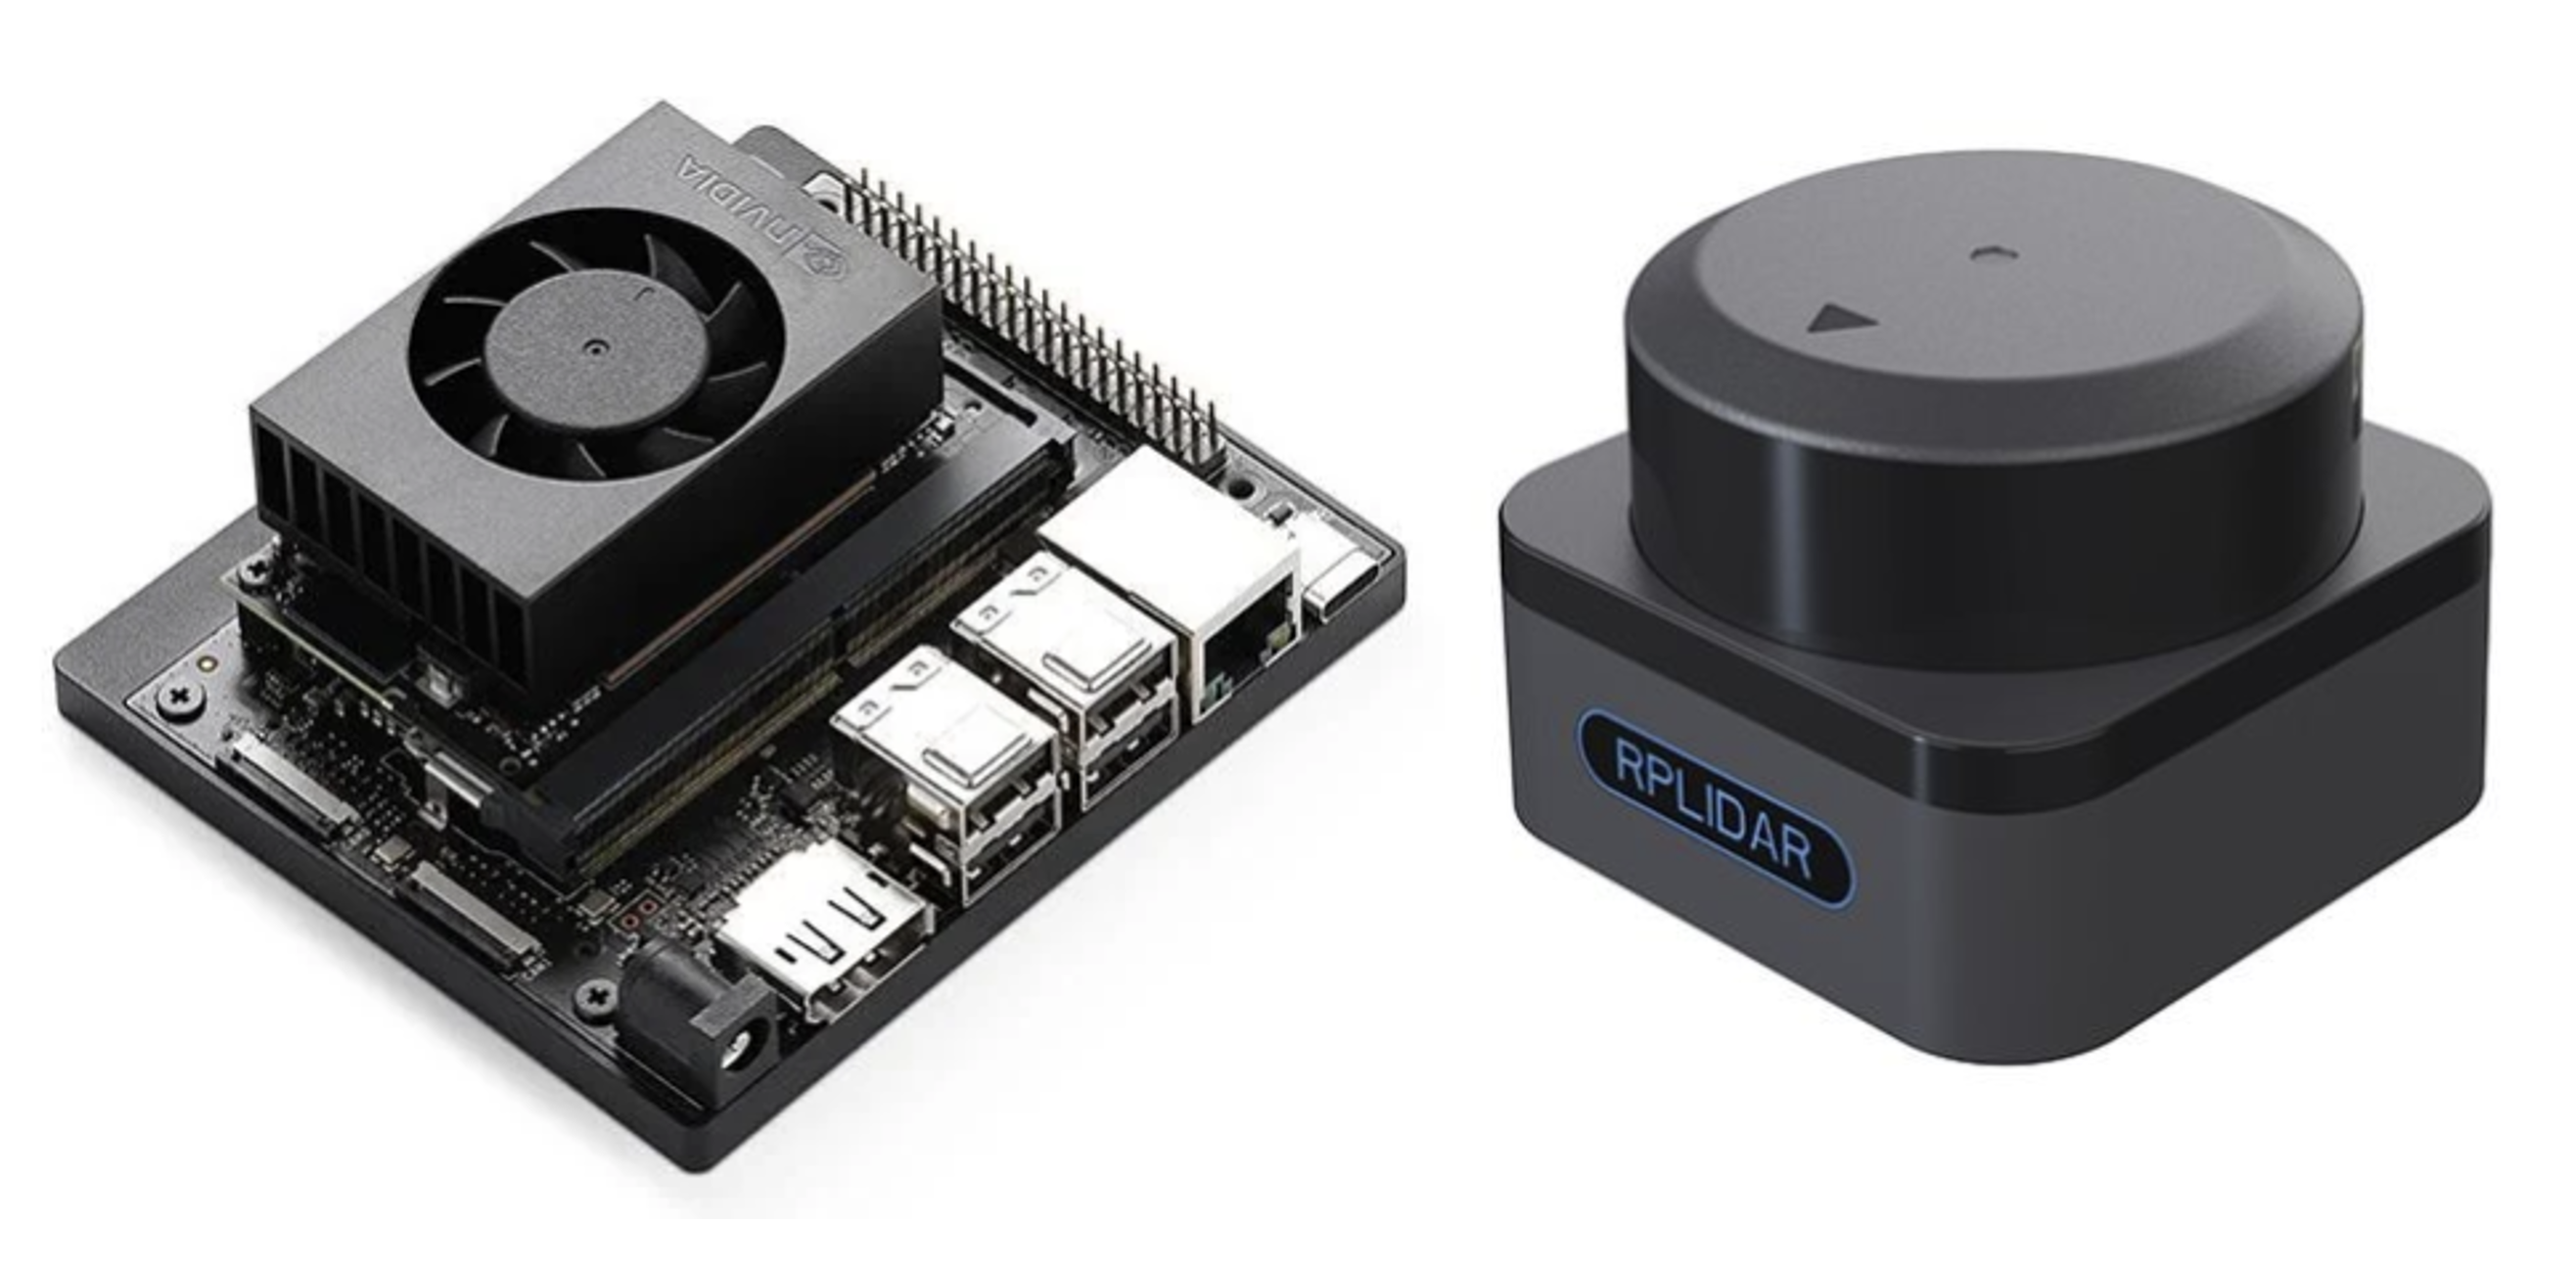
\includegraphics[width=0.5\linewidth]{midpoint_report//assets//images//hardware/JetsonNano+RPLiDAR.png}
    \caption{Image of the Jetson Nano Orin(left) and RPLiDAR S3 360(right)}
    \label{fig:enter-label}
\end{figure}
\paragraph*{}
The next step, after achieving closed-loop control using XDrive with ODrive firmware, is to purchase additional motor drivers and control all four wheels. This will allow us to properly drive the X-Drive omnidirectional system using the Jetson Nano (see \ref{fig:hardware-arch})), which will then be abstracted to operate under ROS.
\begin{figure}
    \centering
    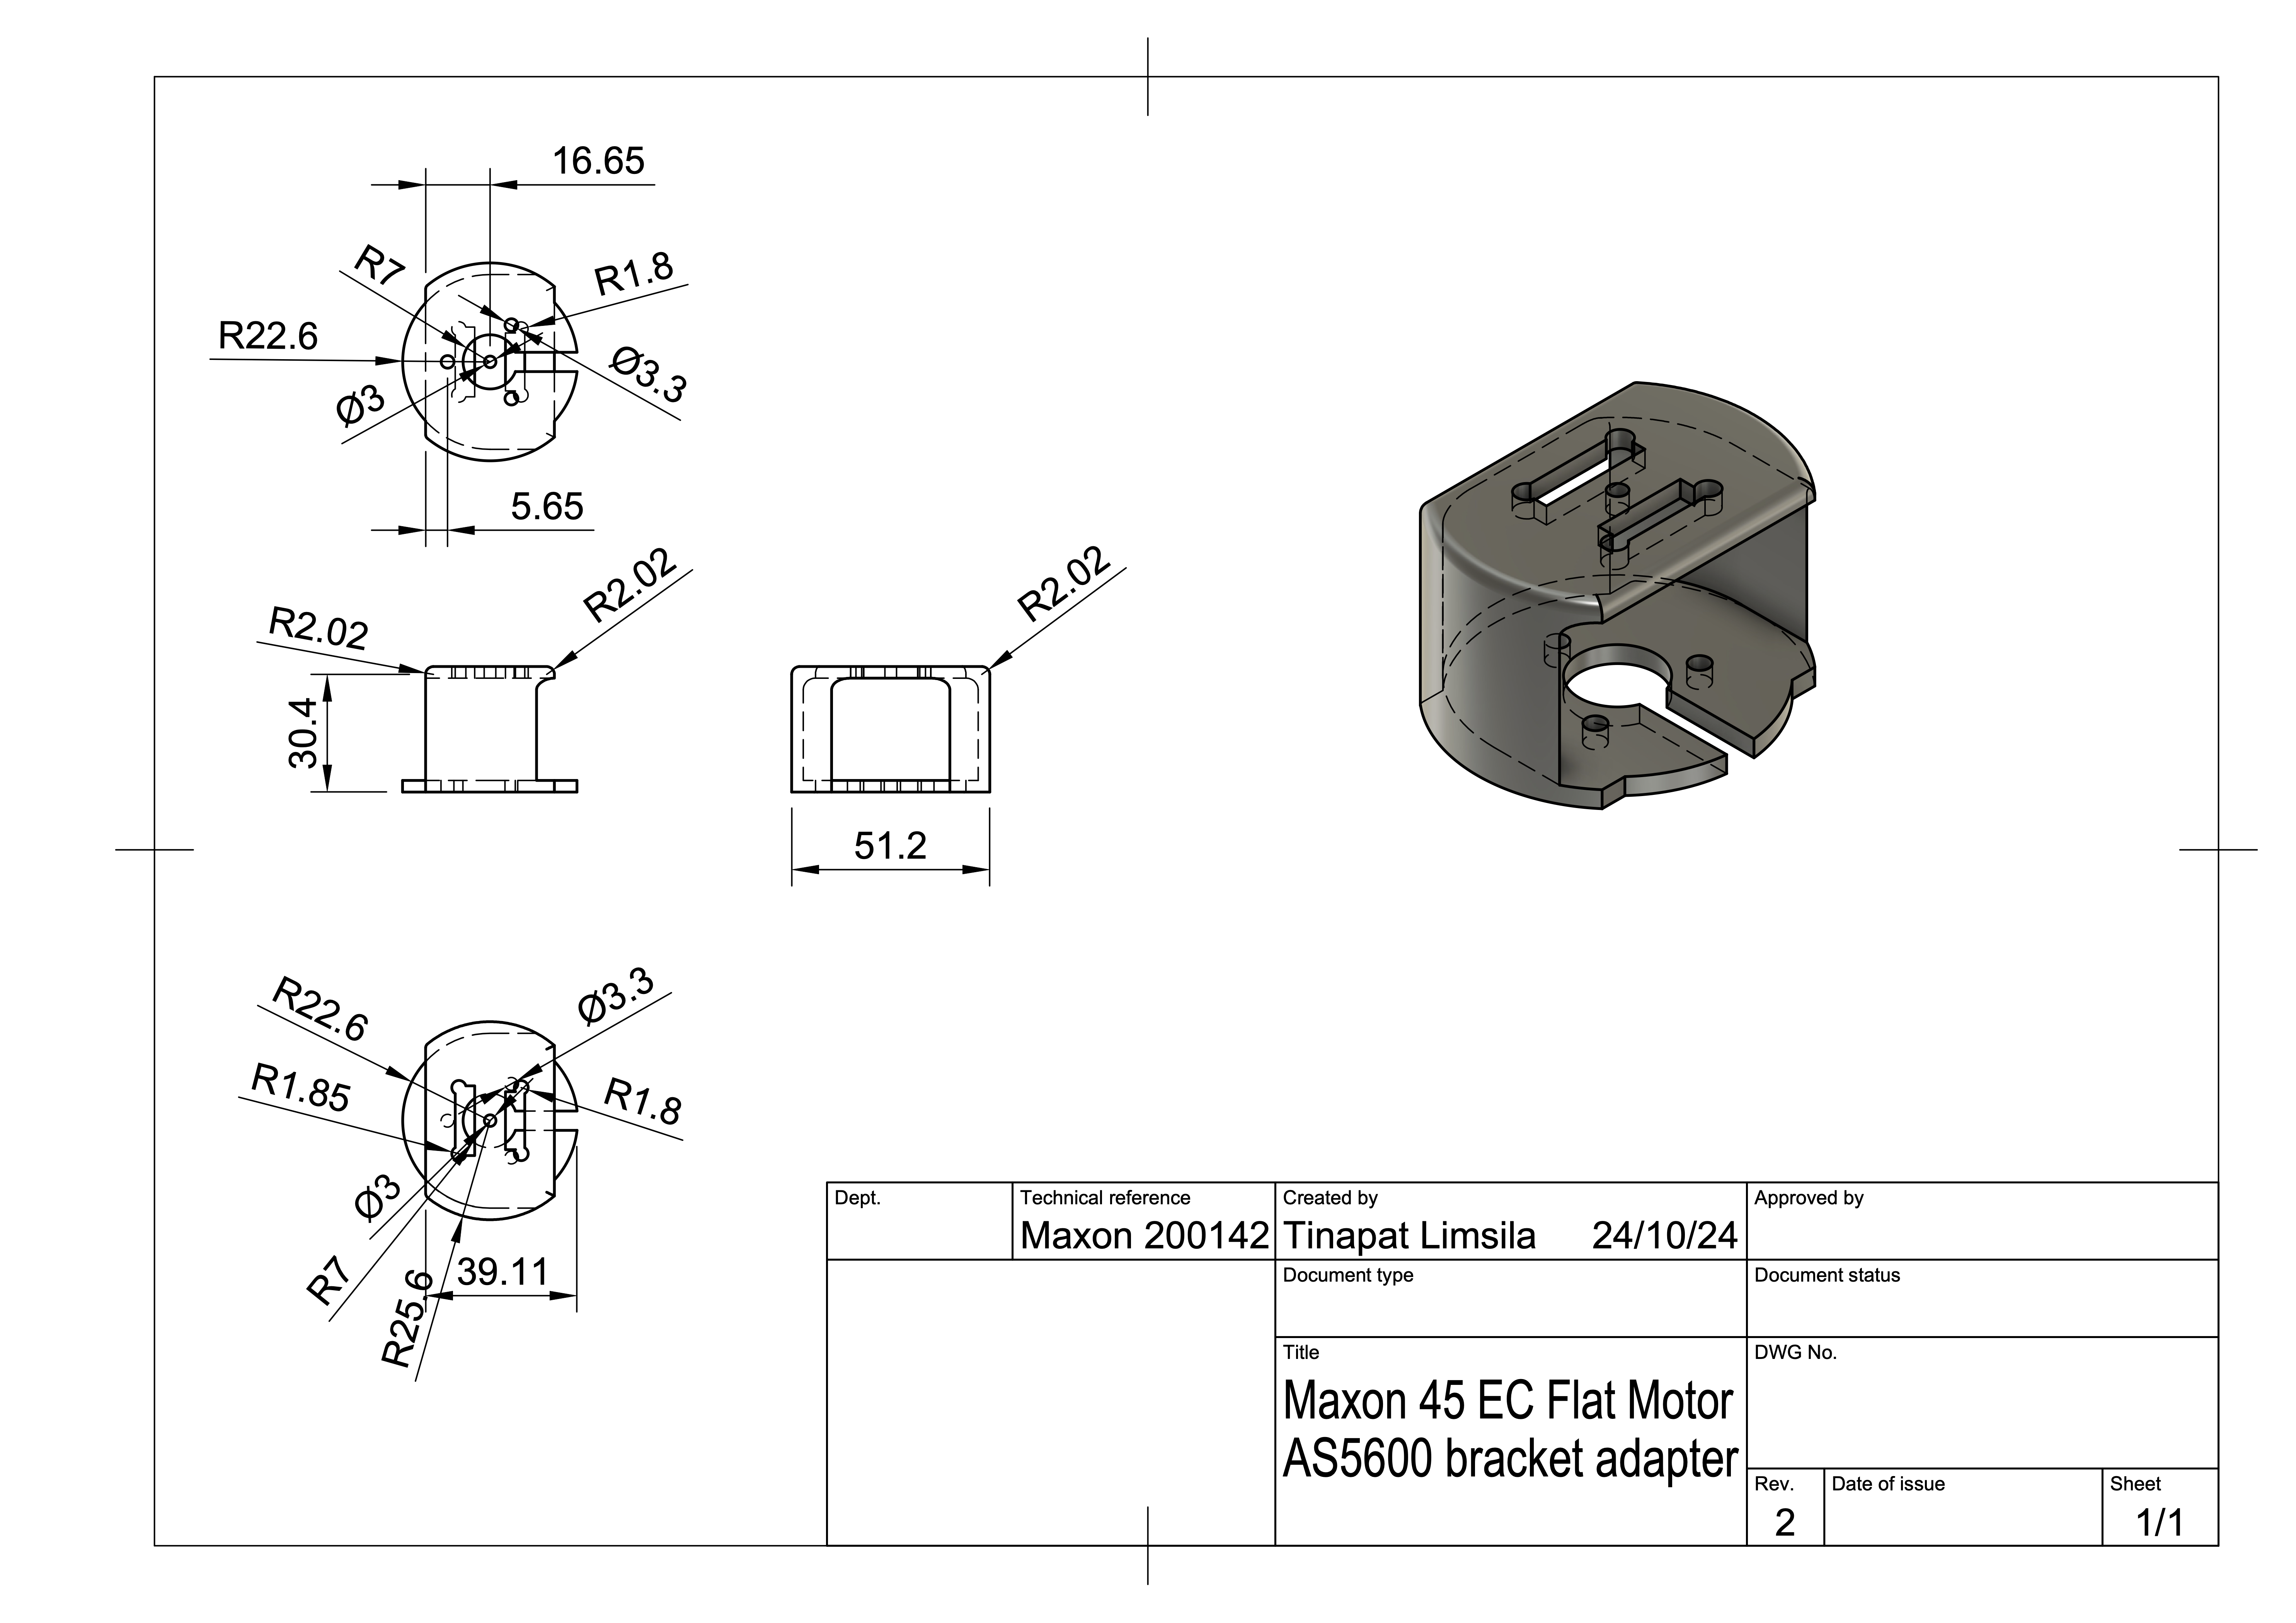
\includegraphics[width=1\linewidth]{assets/images/hardware/Maxon 45 EC Flat Motor AS5600 bracket adapter Drawing v1.png}
    \caption{CAD drawing of the bracket for the Maxon 45 EC Flat motor and the Magnetic Encoder for AS5600}
    \label{fig:real-single-robot}
\end{figure}

\begin{figure}
    \centering
    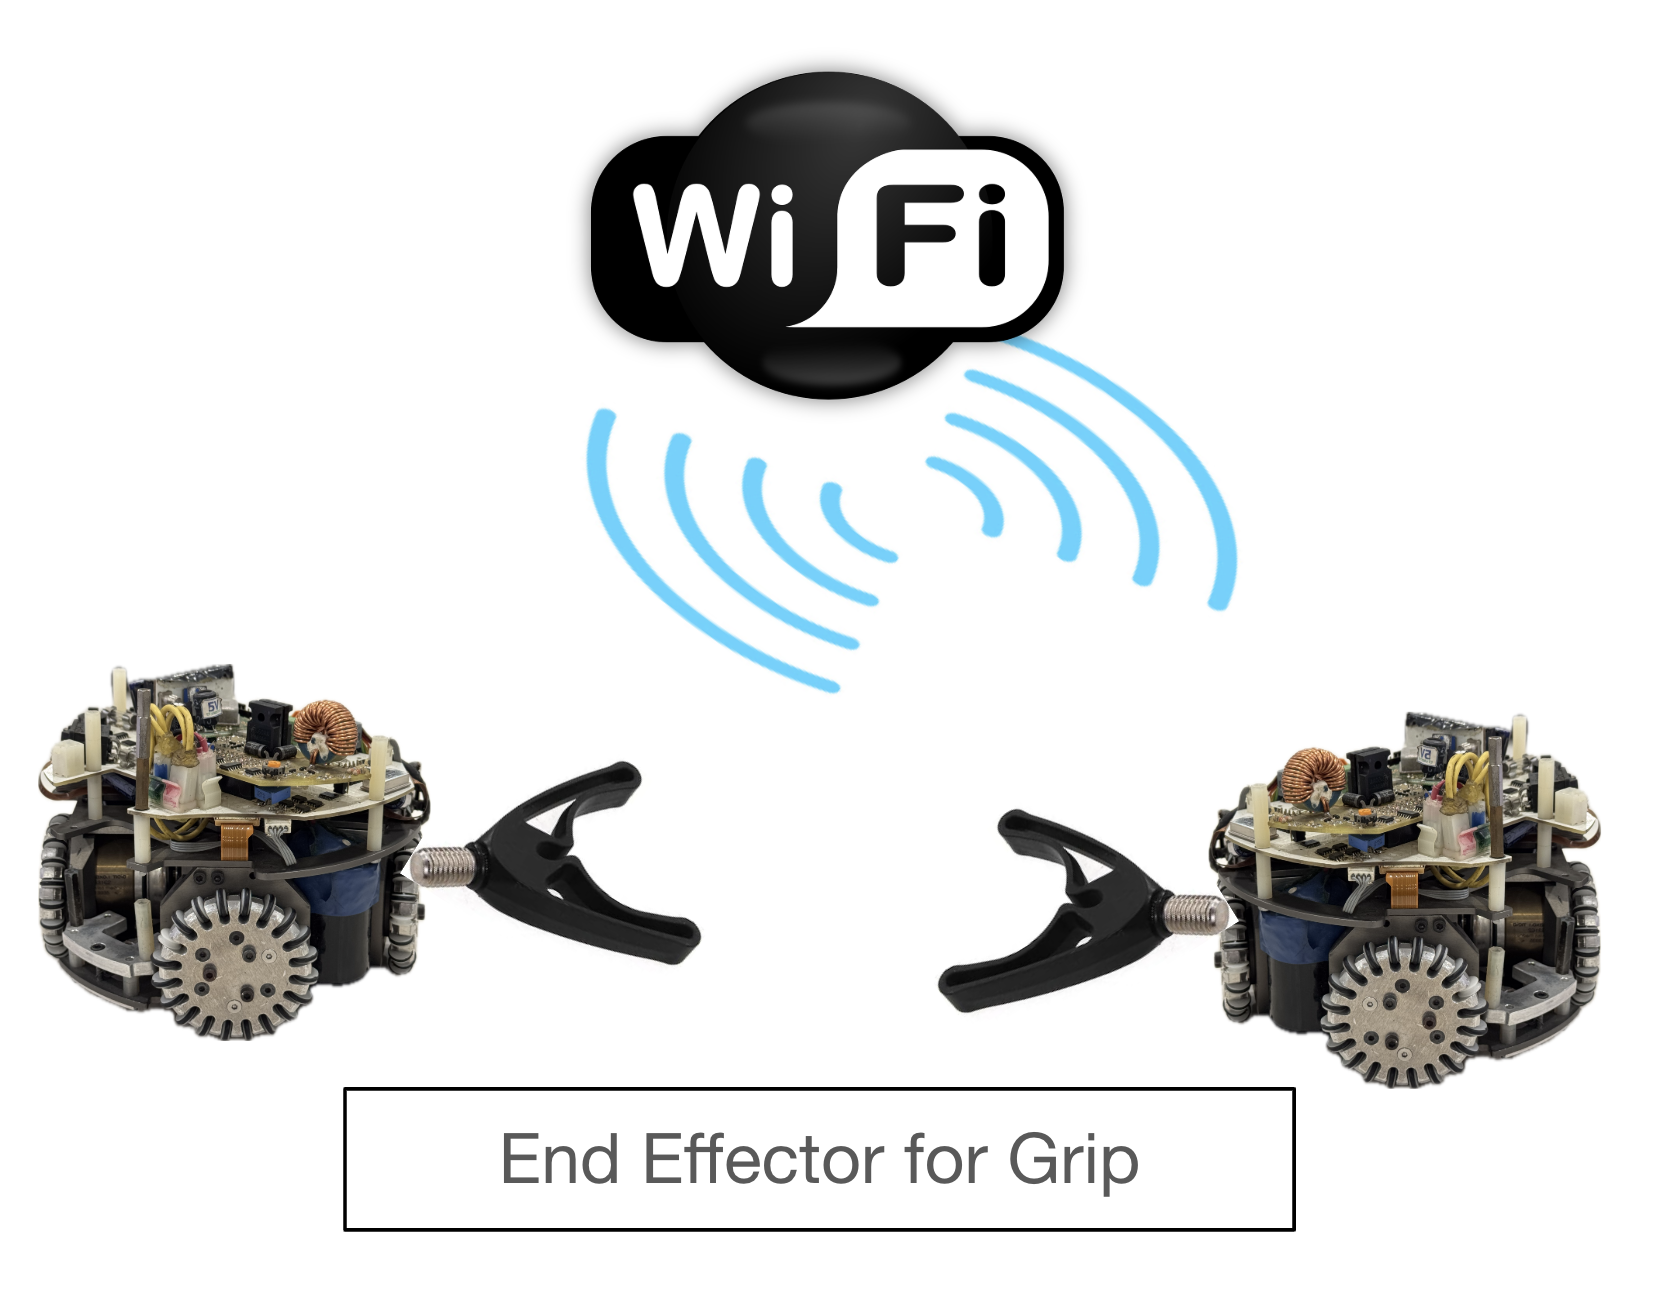
\includegraphics[width=0.5\linewidth]{assets/images/hardware/endeffector.png}
    \caption{Image of the two swarm robot with end effectors with communication via WiFi}
    \label{fig:effector-2-robot}
\end{figure}
\begin{figure}
    \centering
    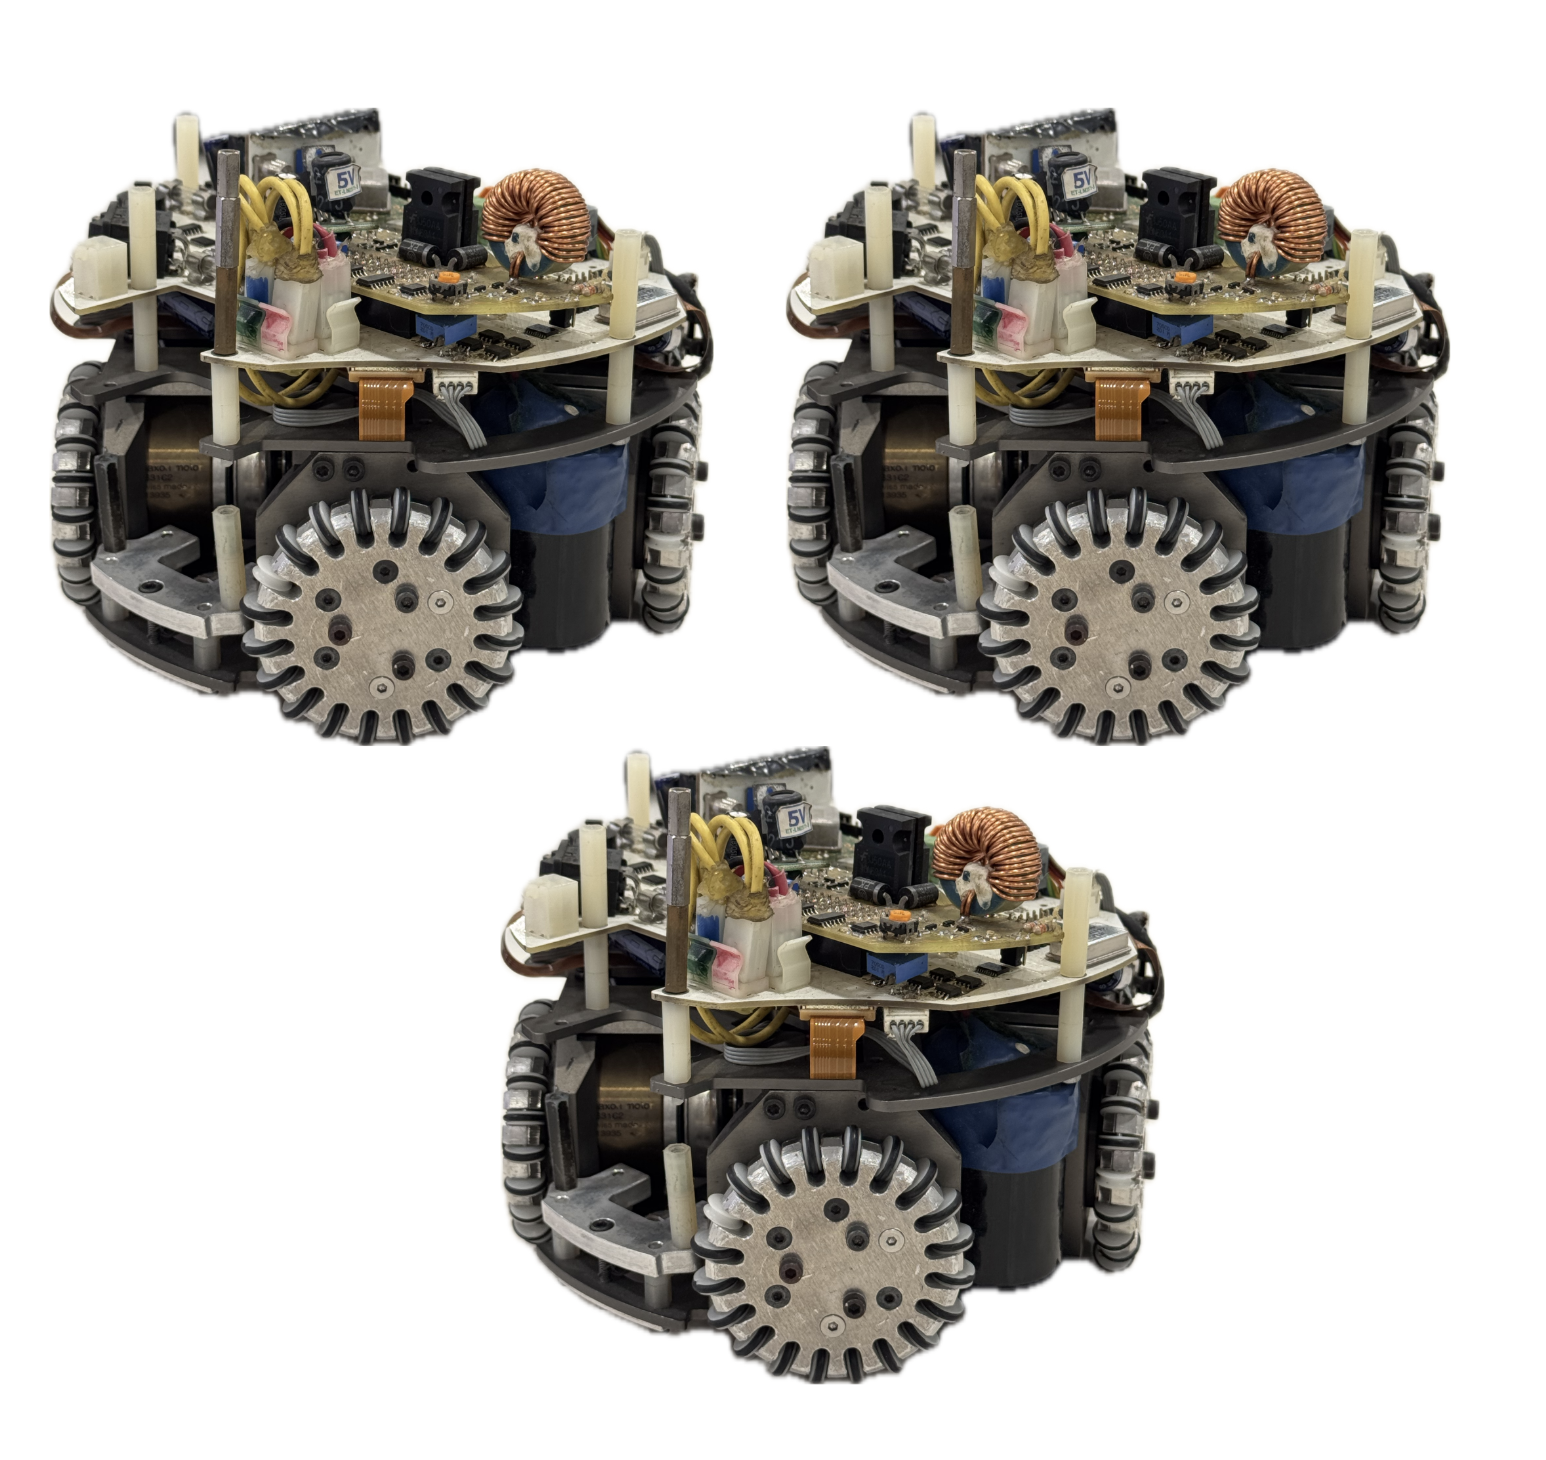
\includegraphics[width=0.5\linewidth]{assets/images/hardware/3swarmrobots.png}
    \caption{Image of the 3 acquired swarm robot pre-modification}
    \label{fig:3-robot}
\end{figure}\begin{figure}
    \centering
    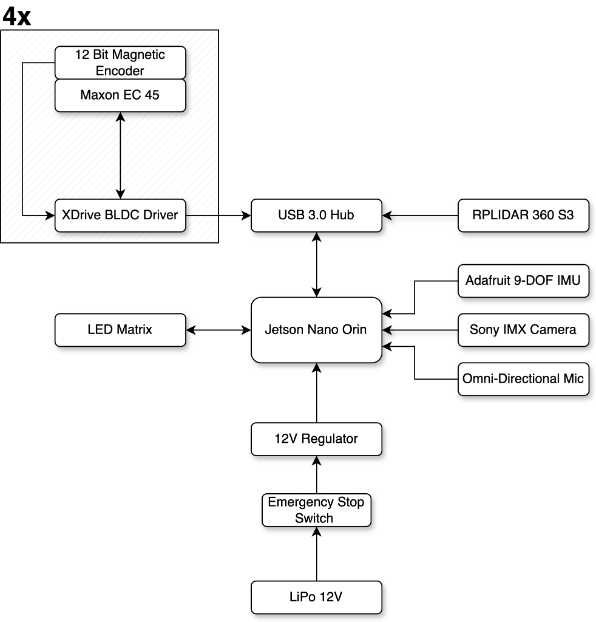
\includegraphics[width=0.75\linewidth]{midpoint_report/assets/images/hardware/hardware-architecture.png}
    \caption{Image of a the hardware architecture and I/O of the system}
    \label{fig:hardware-arch}
\end{figure}

Our hardware in Figure \ref{fig:hardware-arch}, will have safety features such as microphones and an emergency stop button if the robot has software malfunctions. The LED matrix will be the indicator for taskmaster. RPLiDAR 360 S3 will be used for Graph SLAM with the ROS interface package provided. 


% Closing chapters
\chapter{Conclusion}

\paragraph*{}
Swarm communication has been successfully implemented using a decentralized peer-to-peer architecture facilitated by socket communication. This approach was selected for its low latency and reliability, both of which are essential for real-time data exchange among robots. A three-way handshake mechanism was incorporated to ensure message delivery integrity, along with a consensus algorithm to resolve simultaneous object detection and taskmaster assignment conflicts. With coordinate streaming, dynamic path planning, and task execution now fully integrated, the communication system provides a solid foundation for coordinated swarm behavior, enabling seamless transitions between detection, planning, and movement phases.

\paragraph*{}
Additionally, the object detection system utilizing multi-sensor fusion of the camera and S3 RPLiDAR accurately measures relative distance, relative angle, and estimated width, aided by the variation factor function. This function yields an error margin of 1 centimeter for cylinders with diameters of 16 and 20 centimeters. The model was also tested with objects of different sizes, specifically a cylinder with a diameter of 12 centimeters, resulting in a slightly higher error margin of 2 centimeters. Overall, the object detection component was completed within the expected timeline.

\paragraph*{}
For SLAM we will continue making our own graph SLAM but will work on SLAM Toolbox temporarily. For odometry, we will continue testing and publish results soon.

\paragraph*{}
Meanwhile, the development and testing of our holonomic X-Drive robot have progressed significantly. The robot’s base and structural components were 3D printed using PLA, but to improve durability and stability, key parts such as the baseplate, shaft, wheels, and flange coupler will be upgraded to acrylic and stainless steel. The robot utilizes Dynamixel AX-12W motors for enhanced back-drivability, controlled through a custom ROS 2 package that applies a Jacobian matrix transformation for motion control. Transitioning from the older Maxon BLDC motors has streamlined development, allowing us to focus on software for coordinated multi-robot operation. The successful integration of the teleop keyboard package in ROS 2 Humble has demonstrated holonomic movement, paving the way for further improvements in geometry and performance optimization.

\paragraph*{}
For the next phase of our project, we will complete the tasks that have yet to be completed during the previous iteration and move towards a complete swarm. This includes completing the hardware requirements, considering movement after gripping, as well as testing and evaluation. Additionally, we will proceed with other tasks as scheduled in the Gantt Chart to ensure all project milestones are met.

\documentclass{report}
\usepackage{booktabs}
\usepackage{geometry}
\usepackage{caption}
\usepackage{float} % for [H] placement
\geometry{margin=1in}

\begin{document}

\appendix
\chapter{Object Detection Model Testing Result}

\begin{table}[t]
    \centering
    \caption{Predicted diameter under different lighting conditions of 20 cm diameter cylinder, placed at actual relative angle of 0 degree.}
    \label{tab:20cm}
    \begin{tabular}{cccc}
    \toprule
    \textbf{Lighting Condition} & \textbf{Distance (m)} & \textbf{Angle (°)} & \textbf{Predicted Width (m)} \\
    \midrule
    1 & 0.5 & 0.21 & 0.20 \\
    2 & 0.5 & 0.21 & 0.20 \\
    3 & 0.5 & 0.21 & 0.20 \\
    4 & 0.5 & 0.21 & 0.20 \\
    5 & 0.5 & 0.28 & 0.20 \\
    6 & 0.5 & 0.28 & 0.20 \\
    7 & 0.5 & 0.13 & 0.20 \\
    8 & 0.5 & 0.21 & 0.20 \\
    9 & 0.5 & 0.21 & 0.21 \\
    \cmidrule(lr){1-4}
    1 & 1.00 & 0.37 & 0.20 \\
    2 & 1.01 & 0.43 & 0.20 \\
    3 & 1.00 & 0.43 & 0.20 \\
    4 & 1.00 & 0.37 & 0.20 \\
    5 & 1.00 & 0.43 & 0.20 \\
    6 & 1.00 & 0.31 & 0.20 \\
    7 & 1.00 & 0.29 & 0.20 \\
    8 & 1.00 & 0.33 & 0.20 \\
    9 & 1.00 & 0.33 & 0.20 \\
    \cmidrule(lr){1-4}
    1 & 2.00 & 0.18 & 0.20 \\
    2 & 1.99 & 0.18 & 0.20 \\
    3 & 2.00 & 0.18 & 0.20 \\
    4 & 2.00 & 0.18 & 0.20 \\
    5 & 2.00 & 0.18 & 0.20 \\
    6 & 1.99 & 0.18 & 0.20 \\
    7 & 2.00 & 0.18 & 0.20 \\
    8 & 2.00 & 0.18 & 0.20 \\
    9 & 2.00 & 0.18 & 0.20 \\
    \cmidrule(lr){1-4}
    1 & 3.00 & 0.35 & 0.20 \\
    2 & 3.00 & 0.29 & 0.20 \\
    3 & 3.00 & 0.29 & 0.20 \\
    4 & 2.99 & 0.29 & 0.20 \\
    5 & 3.00 & 0.29 & 0.20 \\
    6 & 3.00 & 0.29 & 0.20 \\
    7 & 3.01 & 0.35 & 0.19 \\
    8 & 3.00 & 0.29 & 0.20 \\
    9 & 3.00 & 0.29 & 0.20 \\
    \bottomrule
    \end{tabular}
\end{table}

\begin{table}[htbp]
\centering
\caption{Predicted diameter under different lighting conditions of 16 cm diameter cylinder, placed at actual relative angle of 0 degree.}
\label{tab:16cm}
\begin{tabular}{cccc}
\toprule
\textbf{Lighting Condition} & \textbf{Distance (m)} & \textbf{Angle (°)} & \textbf{Predicted Width (m)} \\
\midrule
1 & 0.5 & 358.11 & 0.16 \\
2 & 0.5 & 358.11 & 0.16 \\
3 & 0.5 & 358.11 & 0.16 \\
4 & 0.5 & 358.05 & 0.16 \\
5 & 0.5 & 358.11 & 0.16 \\
6 & 0.5 & 358.11 & 0.16 \\
7 & 0.5 & 358.11 & 0.16 \\
8 & 0.5 & 358.11 & 0.16 \\
9 & 0.5 & 358.11 & 0.16 \\
\cmidrule(lr){1-4}
1 & 1.00 & 0.18 & 0.16 \\
2 & 1.00 & 0.18 & 0.16 \\
3 & 1.00 & 0.18 & 0.16 \\
4 & 1.00 & 0.18 & 0.16 \\
5 & 1.00 & 0.12 & 0.16 \\
6 & 1.00 & 0.18 & 0.16 \\
7 & 1.00 & 0.12 & 0.16 \\
8 & 1.00 & 0.18 & 0.16 \\
9 & 1.00 & 0.18 & 0.16 \\
\cmidrule(lr){1-4}
1 & 2.00 & 0.55 & 0.16 \\
2 & 2.00 & 0.61 & 0.16 \\
3 & 2.00 & 0.61 & 0.16 \\
4 & 2.00 & 0.61 & 0.16 \\
5 & 2.00 & 0.55 & 0.16 \\
6 & 2.00 & 0.55 & 0.16 \\
7 & 2.00 & 0.55 & 0.16 \\
8 & 2.00 & 0.55 & 0.16 \\
9 & 2.00 & 0.55 & 0.16 \\
\cmidrule(lr){1-4}
1 & 3.00 & 0.22 & 0.16 \\
2 & 3.01 & 0.28 & 0.16 \\
3 & 3.00 & 0.28 & 0.16 \\
4 & 3.00 & 0.22 & 0.17 \\
5 & 3.00 & 0.28 & 0.16 \\
6 & 3.00 & 0.28 & 0.16 \\
7 & 3.00 & 0.28 & 0.17 \\
8 & 3.00 & 0.28 & 0.16 \\
9 & 3.00 & 0.28 & 0.16 \\
\bottomrule
\end{tabular}
\end{table}

\begin{table}[htbp]
\centering
\caption{Predicted diameter under different lighting conditions of 12 cm diameter cylinder, placed at actual relative angles of 2, 0, 1.5, and 0 degrees.}
\label{tab:12cm}
\begin{tabular}{cccc}
\toprule
\textbf{Lighting Condition} & \textbf{Distance (m)} & \textbf{Angle (°)} & \textbf{Predicted Width (m)} \\
\midrule
1 & 0.5 & 2.01 & 0.13 \\
2 & 0.5 & 2.01 & 0.13 \\
3 & 0.5 & 2.01 & 0.12 \\
4 & 0.5 & 2.00 & 0.14 \\
5 & 0.5 & 2.01 & 0.13 \\
6 & 0.5 & 2.01 & 0.12 \\
7 & 0.5 & 2.02 & 0.13 \\
8 & 0.5 & 2.01 & 0.14 \\
9 & 0.5 & 2.01 & 0.13 \\
\cmidrule(lr){1-4}
1 & 1.00 & 0.21 & 0.12 \\
2 & 1.00 & 0.21 & 0.13 \\
3 & 1.00 & 0.20 & 0.13 \\
4 & 1.00 & 0.21 & 0.12 \\
5 & 1.00 & 0.21 & 0.12 \\
6 & 1.01 & 0.23 & 0.14 \\
7 & 1.00 & 0.21 & 0.12 \\
8 & 1.00 & 0.23 & 0.13 \\
9 & 1.00 & 0.21 & 0.13 \\
\cmidrule(lr){1-4}
1 & 2.00 & 1.65 & 0.12 \\
2 & 2.00 & 1.65 & 0.12 \\
3 & 2.01 & 1.68 & 0.12 \\
4 & 2.00 & 1.65 & 0.13 \\
5 & 2.00 & 1.68 & 0.13 \\
6 & 2.00 & 1.65 & 0.12 \\
7 & 2.00 & 1.65 & 0.12 \\
8 & 1.99 & 1.68 & 0.14 \\
9 & 2.00 & 1.68 & 0.14 \\
\cmidrule(lr){1-4}
1 & 3.00 & 0.05 & 0.12 \\
2 & 3.00 & 0.05 & 0.12 \\
3 & 3.00 & 0.05 & 0.14 \\
4 & 3.01 & 0.05 & 0.12 \\
5 & 3.00 & 0.05 & 0.14 \\
6 & 3.00 & 0.05 & 0.13 \\
7 & 3.00 & 0.05 & 0.12 \\
8 & 3.00 & 0.05 & 0.13 \\
9 & 3.00 & 0.05 & 0.12 \\
\bottomrule
\end{tabular}
\end{table}

\end{document}


% Bibliography
\nocite{*}
\printbibliography

\end{document}
